\documentclass[a4paper,12pt]{article}

%=================================================
% ENCODING & LANGUAGE
%=================================================
\usepackage[T1]{fontenc}
\usepackage[utf8]{inputenc}
\usepackage[ngerman]{babel}
\usepackage{csquotes}

%=================================================
% FONTS & MATH
%=================================================
\usepackage{mathptmx}
\usepackage{amsmath}
\usepackage{amssymb}

%=================================================
% GRAPHICS & TABLES
%=================================================
\usepackage{graphicx}
\usepackage[table]{xcolor}
\usepackage{float}
\usepackage{subcaption}
\usepackage{multirow}
\usepackage{multicol}
\usepackage{supertabular}
\usepackage{longtable}
\usepackage{array}
\usepackage{booktabs}
\usepackage{tabularx}
\usepackage{caption}
\captionsetup{labelfont=bf,labelsep=colon,font=small,justification=centering}

\usepackage{eso-pic}
\usepackage{transparent}

%=================================================
% COLORS (Hochschul-Farbschema)
%=================================================
\definecolor{unidark}{HTML}{17365D}
\definecolor{unimid}{HTML}{365F91}
\definecolor{uniaccent}{HTML}{4F81BD}

%=================================================
% HEADING STYLE
%=================================================
\usepackage{titlesec}
\titleformat{\section}{\normalfont\Large\bfseries\color{unimid}}{\thesection}{1em}{}
\titleformat{\subsection}{\normalfont\large\bfseries\color{unimid}}{\thesubsection}{1em}{}
\titleformat{\subsubsection}{\normalfont\normalsize\bfseries\color{unimid}}{\thesubsubsection}{1em}{}

%=================================================
% LAYOUT
%=================================================
\usepackage{geometry}
\geometry{
    a4paper,
    top=3cm,
    bottom=2.5cm,
    left=2.5cm,
    right=2.5cm
}

\usepackage{pdfpages}
\usepackage{parskip}
\usepackage{placeins}
\usepackage[all]{nowidow}

%=================================================
% HEADER / FOOTER
%=================================================
\usepackage{fancyhdr}
\setlength{\headheight}{41pt}

\pagestyle{fancy}
\fancyhf{}

\fancyhead[L]{
\includegraphics[height=0.9cm]{logos/UIREKA_logo_trim.png}}
\fancyhead[R]{
\includegraphics[height=0.9cm]{logos/FUAS_logo_trim.png}}

\fancyfoot[L]{\small\color{unimid}\Kurztitel}
\fancyfoot[C]{}
\fancyfoot[R]{\thepage}

\renewcommand{\headrulewidth}{0.4pt}
\renewcommand{\headrule}{\hbox to\headwidth{\color{unimid}\leaders\hrule height \headrulewidth\hfill}}

%=================================================
% HYPERLINKS
%=================================================
\usepackage{hyperref}

\hypersetup{
    colorlinks=true,
    linkcolor=unimid,
    urlcolor=unimid,
    citecolor=unimid
}

%=================================================
% MATH / UNITS
%=================================================
\usepackage{siunitx}

\sisetup{
    output-decimal-marker={,},
    group-separator={.},
    group-minimum-digits=4,
    per-mode=symbol
}

\newcommand{\prom}{\textperthousand}

%=================================================
% CITATIONS
%=================================================
\usepackage[backend=biber,style=authoryear,citestyle=authoryear,sorting=nyt,maxcitenames=2,uniquename=false,uniquelist=false,dashed=false]{biblatex}
\addbibresource{references.bib}
\DefineBibliographyStrings{ngerman}{andothers={et al\adddot}}


%=================================================
% PLOTS
%=================================================
\usepackage{pgfplots}
\pgfplotsset{compat=1.18}

%=================================================
% LISTS
%=================================================
\usepackage{enumitem}

%=================================================
% TITLE VARIABLES
%=================================================
\newcommand{\Titel}{OFF THE WALL}
\newcommand{\Untertitel}{Der Anlagenring als durchgehender Grün- und Stadtraum}
\newcommand{\Autor}{Marc Graß, Jotyka Karmakar, Büsra Kaynar, Miguel Ureña-Pliego}
\newcommand{\Studiengang}{Master Infrastruktur – Wasser und Verkehr}
\newcommand{\Semester}{Sommersemester 2026}
\newcommand{\Kurztitel}{Grünraum Anlagenring}

\newcommand{\smalltable}{\fontsize{8.5pt}{10.5pt}\selectfont}

%-------------------------------------------------

\begin{document}

\thispagestyle{empty}

\widowpenalty=10000
\clubpenalty=10000
\brokenpenalty=10000

%-------------------------------------------------
% Optional watermark
%-------------------------------------------------

\newcommand\BackgroundPic{
    \put(0,0){
        \parbox[b][\paperheight]{\paperwidth}{
            \vfill
            \centering
            %\transparent{0.06}
            %\includegraphics[width=\paperwidth]{logos/watermark.png}
            \vfill
        }
    }
}

\AddToShipoutPicture*{\BackgroundPic}

%-------------------------------------------------
% Top logos
%-------------------------------------------------

\noindent
\begin{minipage}[t]{0.48\textwidth}

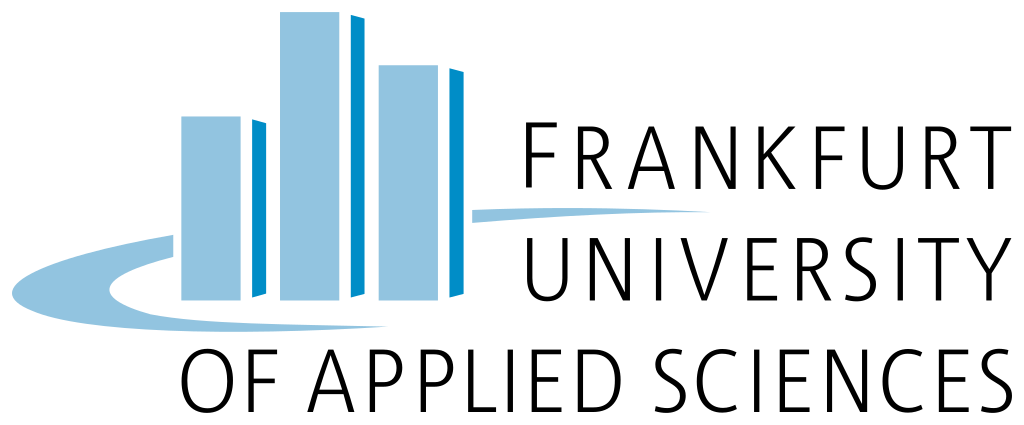
\includegraphics[width=4cm]{logos/FUAS_logo.png}

\end{minipage}
\hfill
\begin{minipage}[t]{0.48\textwidth}

\raggedleft


\includegraphics[width=4cm]{logos/THM_logo.png}

\end{minipage}

\vspace{2cm}

%-------------------------------------------------
% Title
%-------------------------------------------------

\begin{center}

{\Huge\bfseries \Titel}

\vspace{0.7cm}

{\Large \Untertitel}

\end{center}

\vspace{2cm}

%-------------------------------------------------
% Main image
%-------------------------------------------------

\begin{center}

\includegraphics[
width=0.70\textwidth,
keepaspectratio
]{figures/imagen_portada.png}

\end{center}

%-------------------------------------------------
% Information
%-------------------------------------------------

\begin{flushleft}

\textbf{Autor}

\Autor

\textbf{Studiengang}

\Studiengang

\textbf{Semester}

\Semester

\end{flushleft}

\vfill

%-------------------------------------------------
% Universities
%-------------------------------------------------

\begin{center}

Frankfurt University of Applied Sciences und 
Technische Hochschule Mittelhessen
\end{center}

\clearpage

\clearpage

\tableofcontents

\clearpage

\renewcommand{\listfigurename}{Abbildungsverzeichnis}
\listoffigures

\renewcommand{\listtablename}{Tabellenverzeichnis}
\listoftables

\clearpage

\section{Wahrnehmungsumfrage}

\subsection{Hintergrund und Motivation}

Zu erfassen, wie Menschen die Straßen wahrnehmen, auf denen sie gehen, Rad fahren oder sich aufhalten, ist mit klassischen Befragungen schwer zu leisten, da verbale oder numerische Bewertungen von \enquote{Sicherheit} oder \enquote{Schönheit} stark subjektiv und zwischen Befragten kaum vergleichbar sind \autocite{salesses2013}. Eine etablierte Alternative, die durch das Place-Pulse-Projekt des MIT Media Lab bekannt wurde, besteht darin, den Teilnehmenden eine deutlich einfachere Frage zu stellen: Welches von zwei Straßenraumfotos wirkt sicherer, besser begehbar oder einladender? Paarvergleiche dieser Art sind kognitiv leichter zu beantworten, robuster gegenüber individuellen Bewertungsskalen und lassen sich zu einem kontinuierlichen, intervallskalierten Wahrnehmungswert für jedes Bild im Datensatz aggregieren \autocite{salesses2013,naik2014}. Dieser Ansatz wurde inzwischen auf große, mehrere Städte umfassende Straßenraum-Bilddatensätze übertragen, die mit kontextuellen und semantischen Metadaten angereichert sind, um genau solche Analysen der urbanen Wahrnehmung in großem Maßstab zu unterstützen \autocite{hou2024}, und er bildet die Grundlage datengetriebener Pipelines, die menschliche Ortswahrnehmung direkt aus Straßenraumbildern lernen und vorhersagen \autocite{zhang2018}.

Unser Projekt überträgt dasselbe Paradigma auf eine konkrete planerische Fragestellung: Wie nehmen Anwohnende und Besuchende unterschiedliche Straßenraum-Gestaltungsvarianten am Anlagenring in Frankfurt am Main und dessen Umgebung wahr, insbesondere im Hinblick auf Zufußgehen, Radfahren und Aufenthalten im Straßenraum? Wir haben dazu eine webbasierte AB-Testing-Umfrageplattform (\enquote{ABsurveys}) entwickelt, die Teilnehmenden wiederholt zwei Fotografien oder Visualisierungen von Straßenabschnitten zeigt und sie bittet, diejenige auszuwählen, die sie für eine bestimmte Aktivität als angenehmer empfinden. Im Hintergrund der Oberfläche wirken drei Komponenten zusammen, um die Umfrage effizient und ihre Ergebnisse statistisch belastbar zu machen. Erstens eine auf TrueSkill basierende Bewertungs-Engine, die jede binäre Entscheidung in einen aktualisierten, unsicherheitsbehafteten Wahrnehmungswert für jedes Bild umrechnet. Zweitens ein Active-Sampling-Algorithmus zur Paarauswahl, der entscheidet, welche zwei Bilder als Nächstes gezeigt werden, damit die Aufmerksamkeit der Teilnehmenden dort eingesetzt wird, wo sie den größten Informationsgewinn liefert. Drittens ein StreetScore-artiges Deep-Learning-Modell, das die menschlichen Vergleiche auf die deutlich größere Menge an Bildern verallgemeinert, die nie direkt bewertet wurden. Dieser Bericht erläutert, wie diese drei Komponenten funktionieren, und fasst ihren Einsatz an unserem Reallabor-Tag am Anlagenring zusammen.

Konzeptionelles Vorbild für unsere Plattform ist \enquote{Place Pulse} des MIT Media Lab, das denselben paarweisen Vergleichsansatz erstmals in großem Maßstab für die Wahrnehmung von Straßenräumen eingesetzt hat und unter \url{https://cs-futurecities.media.mit.edu/} weiterhin einsehbar ist \autocite{salesses2013,naik2014}. Abbildung~\ref{fig:survey-web} zeigt die Weboberfläche unserer eigenen, daran angelehnten Umfrageplattform \enquote{ABsurveys}, wie sie sowohl am Vor-Ort-Computer als auch über den ausgehängten QR-Code auf dem eigenen Smartphone genutzt werden konnte.

\begin{figure}[H]
	\centering
	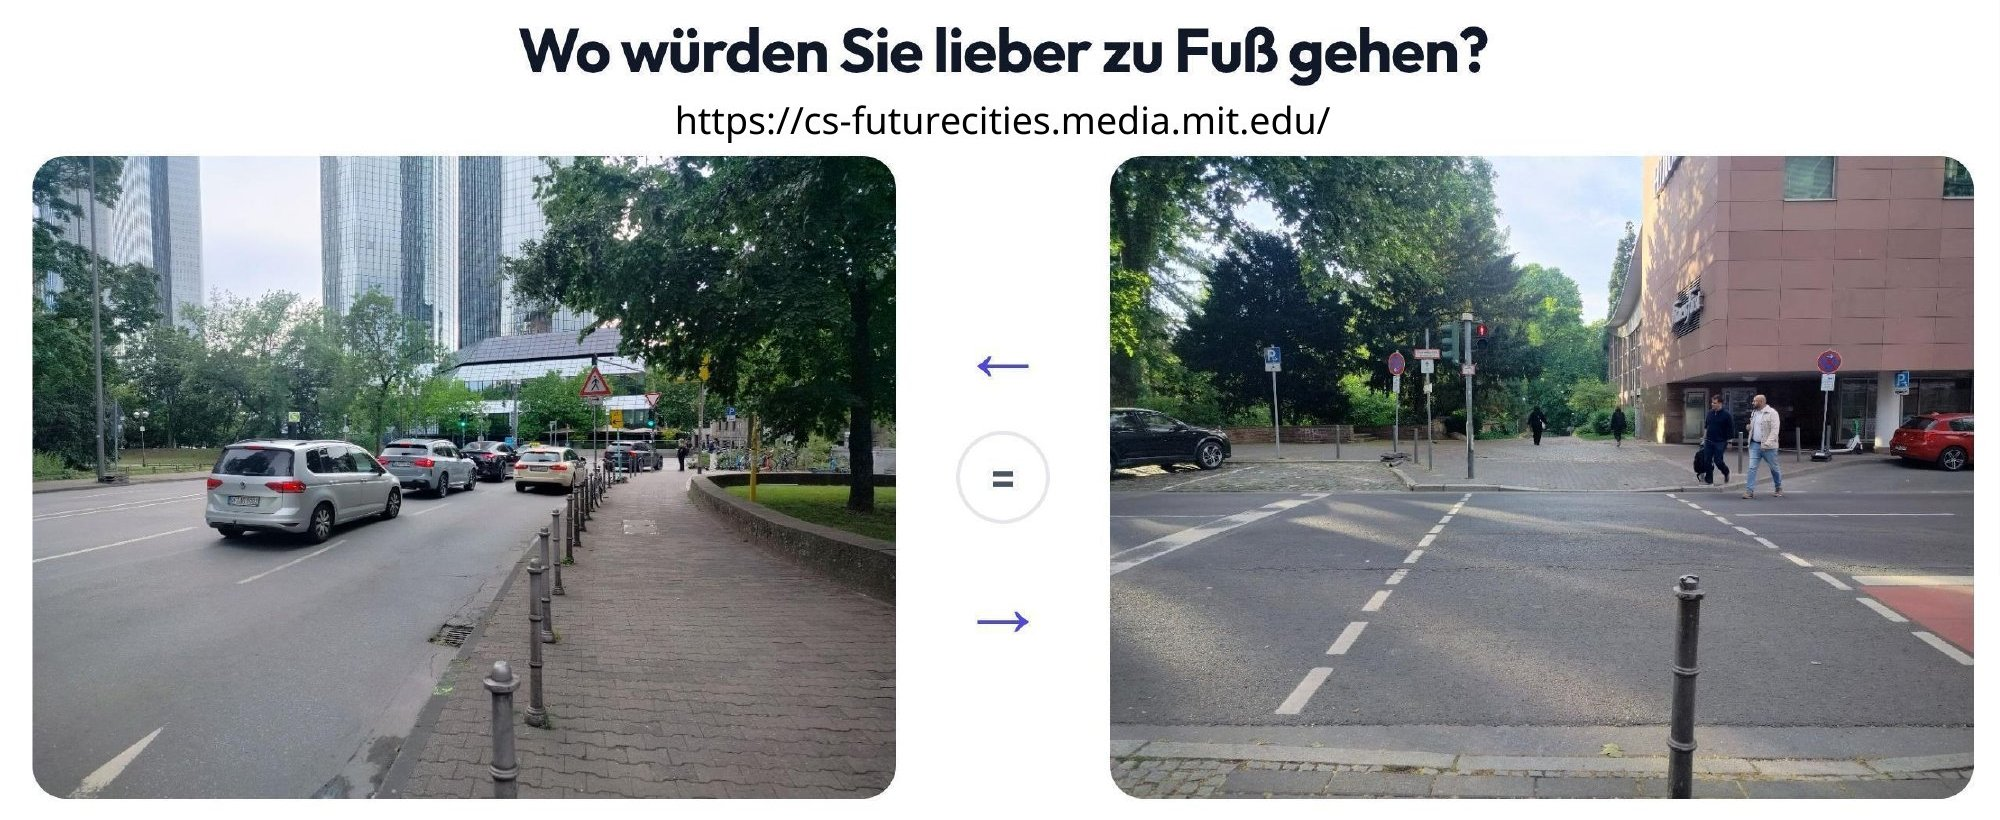
\includegraphics[width=0.7\textwidth]{figures/survey_web.jpg}
	\caption[Weboberfläche der ABsurveys-Umfrageplattform]{Screenshot der Weboberfläche der ABsurveys-Umfrageplattform (Quelle: eigene Darstellung).}
	\label{fig:survey-web}
\end{figure}

\subsection{Paarvergleich als Messinstrument}

Statt zu fragen \enquote{Wie sicher ist diese Straße auf einer Skala von 1--10?}, zeigt die Plattform zwei Bilder nebeneinander und erfasst nur ein dreistufiges Ergebnis (A bevorzugt, B bevorzugt oder unentschieden). Diese Gestaltungsentscheidung folgt unmittelbar aus der psychometrischen Literatur zum vergleichenden Urteilen: Relative Urteile zwischen zwei Stimuli sind weniger anfällig für Ankereffekte und Skaleninterpretationsverzerrungen als absolute Bewertungen, und sie erlauben es, viele unabhängige, mit geringem Aufwand abgegebene Antworten verschiedener Nutzender zu einer gemeinsamen Rangfolge zusammenzuführen \autocite{salesses2013}. Dieselbe Logik liegt großen Citizen-Science-Plattformen zur Wahrnehmungserhebung wie Place Pulse zugrunde, die weltweit Millionen paarweiser Urteile (\enquote{sicherer/lebendiger/schöner}) zu Straßenraumbildern sammelten und daraus bildbezogene Wahrnehmungswerte ableiteten \autocite{salesses2013,naik2014}. In unserer Umfrage ist jeder Vergleich einer bestimmten Aktivität (Gehen, Radfahren oder Aufenthalten) sowie einer bestimmten Bildkategorie zugeordnet (z.\,B. unterschiedliche Arten der Trennung zwischen Rad- und Kfz-Verkehr), sodass die resultierenden Wahrnehmungswerte später als aktivitätsspezifische Indikatoren für die Straßenraumqualität interpretiert werden können und nicht als ein einziger, allgemeiner \enquote{Schönheits}-Wert.

\subsection{Von Entscheidungen zu Werten: TrueSkill}

Eine einzelne paarweise Entscheidung sagt für sich genommen nur aus, dass ein Bild einem anderen vorgezogen wurde; sie ergibt noch keinen numerischen Wert. Um einen wachsenden Strom solcher Vergleiche in stabile, vergleichbare Werte zu überführen, nutzt die Plattform TrueSkill, ein von Microsoft Research entwickeltes bayessches Bewertungssystem zur Einstufung von Spielenden in Online-Mehrspielerspielen anhand einzelner Partieergebnisse \autocite{herbrich2007}. Jedes Bild wird als Gaußverteilung über seine wahrgenommene Qualität für eine Aktivität dargestellt:

\[
\text{Bild}_i \sim \mathcal{N}(\mu_i, \sigma_i^2)
\]

\begin{itemize}
	\item $\mu$ ist die aktuell beste Schätzung des Wahrnehmungswerts.
	\item $\sigma$ (\enquote{Uncertainty}) gibt an, wie sicher diese Schätzung ist. Der Wert ist groß bei wenigen und klein bei vielen Vergleichen.
\end{itemize}

Nach jedem AB-Vergleich läuft folgender Zyklus ab:

\begin{enumerate}
	\item Beide Bilder werden als TrueSkill-Ratings $(\mu_A,\sigma_A)$, $(\mu_B,\sigma_B)$ geladen.
	\item Ein approximatives bayessches Update (Message-Passing auf einem Faktorgraphen) verschiebt $\mu$ des gewählten Bildes nach oben und $\mu$ des abgelehnten nach unten. Das Ausmaß der Verschiebung ist proportional dazu, wie überraschend das Ergebnis angesichts der bisherigen Ratings war.
	\item Beide $\sigma$-Werte werden leicht reduziert, da ein zusätzlicher Beleg vorliegt.
	\item Die neuen Werte werden persistiert und stehen sofort für die nächste Paarauswahl zur Verfügung.
\end{enumerate}

Anders als eine statische Rangliste, die erst am Ende der Erhebung berechnet wird, aktualisiert TrueSkill Werte und Uncertainty online nach jedem Klick \autocite{herbrich2007}. Zwei Größen aus diesem Zustand werden weiterverwendet: $\sigma$ steuert das Active Sampling (Abschnitt~\ref{sec:active-sampling}), und sobald $\sigma$ für $\geq 90\,\%$ der aktiven Bilder unter einem Schwellenwert liegt, wird der Bildpool um eine neue, zuvor zurückgehaltene Charge erweitert (Curriculum-Strategie).

\subsection{Entscheiden, was als Nächstes gezeigt wird: Active Sampling}
\label{sec:active-sampling}

Bei mehreren hundert Bildern über drei Aktivitäten hinweg ist es weder praktikabel, jedem Teilnehmenden jedes mögliche Bildpaar zu zeigen, noch effizient, Paare rein zufällig auszuwählen. Die Plattform nutzt daher Active Sampling im Sinne des poolbasierten aktiven Lernens: Aus einem Kandidatenpool wird das Element mit dem größten erwarteten Informationsgewinn ausgewählt, statt passiv zufällig zu stichproben \autocite{settles2009}. Die Paarauswahl folgt drei Kriterien, kombiniert in einem Informationsgewinn-Score:

\begin{table}[H]
	\centering
	\begin{tabularx}{\textwidth}{@{}llX@{}}
		\toprule
		Kriterium & Gewicht & Idee \\
		\midrule
		Uncertainty $\sigma$ & 0.5 & Bilder mit unsicherem Rating werden bevorzugt gezeigt \\
		Score-Ähnlichkeit & 0.3 & Vergleiche zwischen ähnlich bewerteten Bildern sind am aussagekräftigsten \\
		Novität (wenig gesehen) & 0.2 & Selten gezeigte Bilder werden bevorzugt \\
		\bottomrule
	\end{tabularx}
	\caption[Kriterien des Informationsgewinn-Scores]{Kriterien des Informationsgewinn-Scores beim Active Sampling (Quelle: eigene Darstellung).}
\end{table}

Das Ankerbild wird mit einer zu $\sigma$ proportionalen Wahrscheinlichkeit gezogen. Sein Vergleichspartner wird aus den Top-Kandidaten nach obigem Score gezogen \autocite{settles2009}. Ein Parameter mischt diese unsicherheitsgetriebene Auswahl mit rein zufälliger Ziehung, sodass sich der Grad der \enquote{Aktivität} je Einsatz justieren lässt. Zusätzliche harte Regeln (keine wiederholten Paare/Bilder pro Person, keine inkompatiblen Paare, Cold-Start-Exploration ungesehener Bilder zuerst) stellen sicher, dass die Abfolge sowohl statistisch effizient als auch für Nutzende angenehm bleibt.

\subsection{Verallgemeinerung über die abgefragten Bilder hinaus: StreetScore \& Fine-Tuning}

Selbst mit Active Sampling bleibt die Zahl direkt verglichener Bilder klein gegenüber der Zahl an Straßenabschnitten, die am Ende bewertet werden sollen. Das Vorbild dafür ist StreetScore: \textcite{naik2014} trainierten anhand mehrerer Millionen crowdgesourcter Paarvergleiche auf über einer Million Straßenansichten weltweit (gesammelt über Place Pulse) ein Modell, das die wahrgenommene Sicherheit von Straßenbildern vorhersagt, die nie von einer teilnehmenden Person bewertet wurden. Wir übernehmen diese Grundidee, ersetzen die ursprüngliche Merkmals-/SVR-Architektur jedoch durch einen moderneren Vision Transformer (ViT-B/16) \autocite{dosovitskiy2021}, wie er in einer aktuellen, auf dem Place-Pulse-Datensatz pretrainierten Streetscore-Neuimplementierung für menschliche Ortswahrnehmung eingesetzt wird \autocite{hou2024}.

Dieses pretrainierte Modell lieferte auf unseren Bildern jedoch keine verlässlichen Vorhersagen. Der wahrscheinliche Grund: Es wurde auf weltweit über Google Street View gesammelten Bildern trainiert, die überwiegend befahrene Straßen mit Fahrzeugen zeigen, während unsere Aufnahmen Park- und Fußwegbereiche am Anlagenring abbilden, in denen Straßen und Autos meist gar nicht sichtbar sind. Es handelt sich damit um eine deutliche Domänenverschiebung. Wir haben deshalb eine eigene Fine-Tuning-Schleife implementiert, die das Modell auf unsere lokal erhobenen Paarvergleiche nachtrainiert, sodass es lernt, wie unsere befragten Bürgerinnen und Bürger zu urteilen:

\begin{enumerate}
	\item Export der TrueSkill-Paarvergleiche aus der Feldstudie als Trainingsdaten.
	\item Bildseitiger Split (train/val/test), sodass kein Bild in mehreren Splits gleichzeitig auftaucht.
	\item Fine-Tuning des ViT-Encoders + MLP-Kopfs mit einem differenzierbaren paarweisen Ranking-Verlust, der das vorhergesagte Rating des bevorzugten Bildes über das des abgelehnten drückt, statt Vergleiche vorab in künstliche Einzel-Labels umzuwandeln.
	\item Auswertung mittels Pair-Accuracy sowie einer dualen Uncertainty (Entropie- und Monte-Carlo-Dropout-basiert), um Vorhersagen für unserer Trainingsdomäne ähnliche Straßenabschnitte von denen in visuell unbekannten Gebieten zu unterscheiden.
\end{enumerate}

Dieser Fine-Tuning-Schritt ist damit nicht nur eine Übertragung des Streetscore-Prinzips auf modernere Architekturen (vgl. \textcite{hou2024} zur wachsenden Verfügbarkeit standardisierter Straßenraum-Bilddaten für solche Transferaufgaben), sondern vor allem die notwendige Anpassung an eine Bilddomäne (autofreie Park- und Fußwegräume), die von den ursprünglichen, weltweit auf Straßenverkehr fokussierten Trainingsdaten kaum abgedeckt wird.

\subsection{Anwendung im Feld: Der Reallabor-Tag am Anlagenring}

Der oben beschriebene dreiteilige Mechanismus wurde für eine konkrete Fallstudie am Anlagenring, dem entlang der ehemaligen Stadtbefestigung verlaufenden Ring in Frankfurt am Main, sowie dessen Umgebungsstraßen eingesetzt. Wir haben an 138 Standorten entlang des Anlagenrings und angrenzender Straßen Straßenraumfotografien aufgenommen, die eine Bandbreite bestehender und möglicher Gestaltungsvarianten für die Bedingungen des Gehens, Radfahrens und Aufenthaltens abdecken. Da dieselbe Aufnahme teils für mehrere Aktivitätskategorien relevant ist, ergeben sich daraus 239 Bild-Einträge im Umfrage-Pool (91 Geh-, 91 Rad- und 56 Aufenthalts-Einträge plus 2 Einstiegsbilder). An unserem Reallabor-Feldtag wurde die Umfrage in zwei parallelen Zugängen durchgeführt: vor Ort an einem einzelnen aufgestellten Computer, an dem Anwohnende und Passanten direkt teilnehmen konnten, sowie zusätzlich über einen ausgehängten QR-Code, der auf dieselbe Web-Version der Umfrage verlinkte und so eine Teilnahme über das eigene Smartphone ermöglichte. Über beide Zugänge zusammen nahmen 27 Befragte teil (18 am Vor-Ort-Computer, 9 über den QR-Code/Web-Zugang) und erzeugten dabei 912 paarweise Klicks über die Kategorien Gehen, Radfahren und Aufenthalten hinweg, die live in die TrueSkill-Bewertungs-Engine einflossen und zur Aktualisierung der Wahrnehmungswerte sowie der oben beschriebenen StreetScore-Trainingsdaten genutzt wurden. Diese Werte bilden zusammen mit den zugehörigen Uncertainties die empirische Grundlage für die Wahrnehmungskarten und Vergleichsanalysen, die im weiteren Verlauf dieses Berichts vorgestellt werden.

\subsection{Ergebnisse}

\begin{figure}[H]
	\centering
	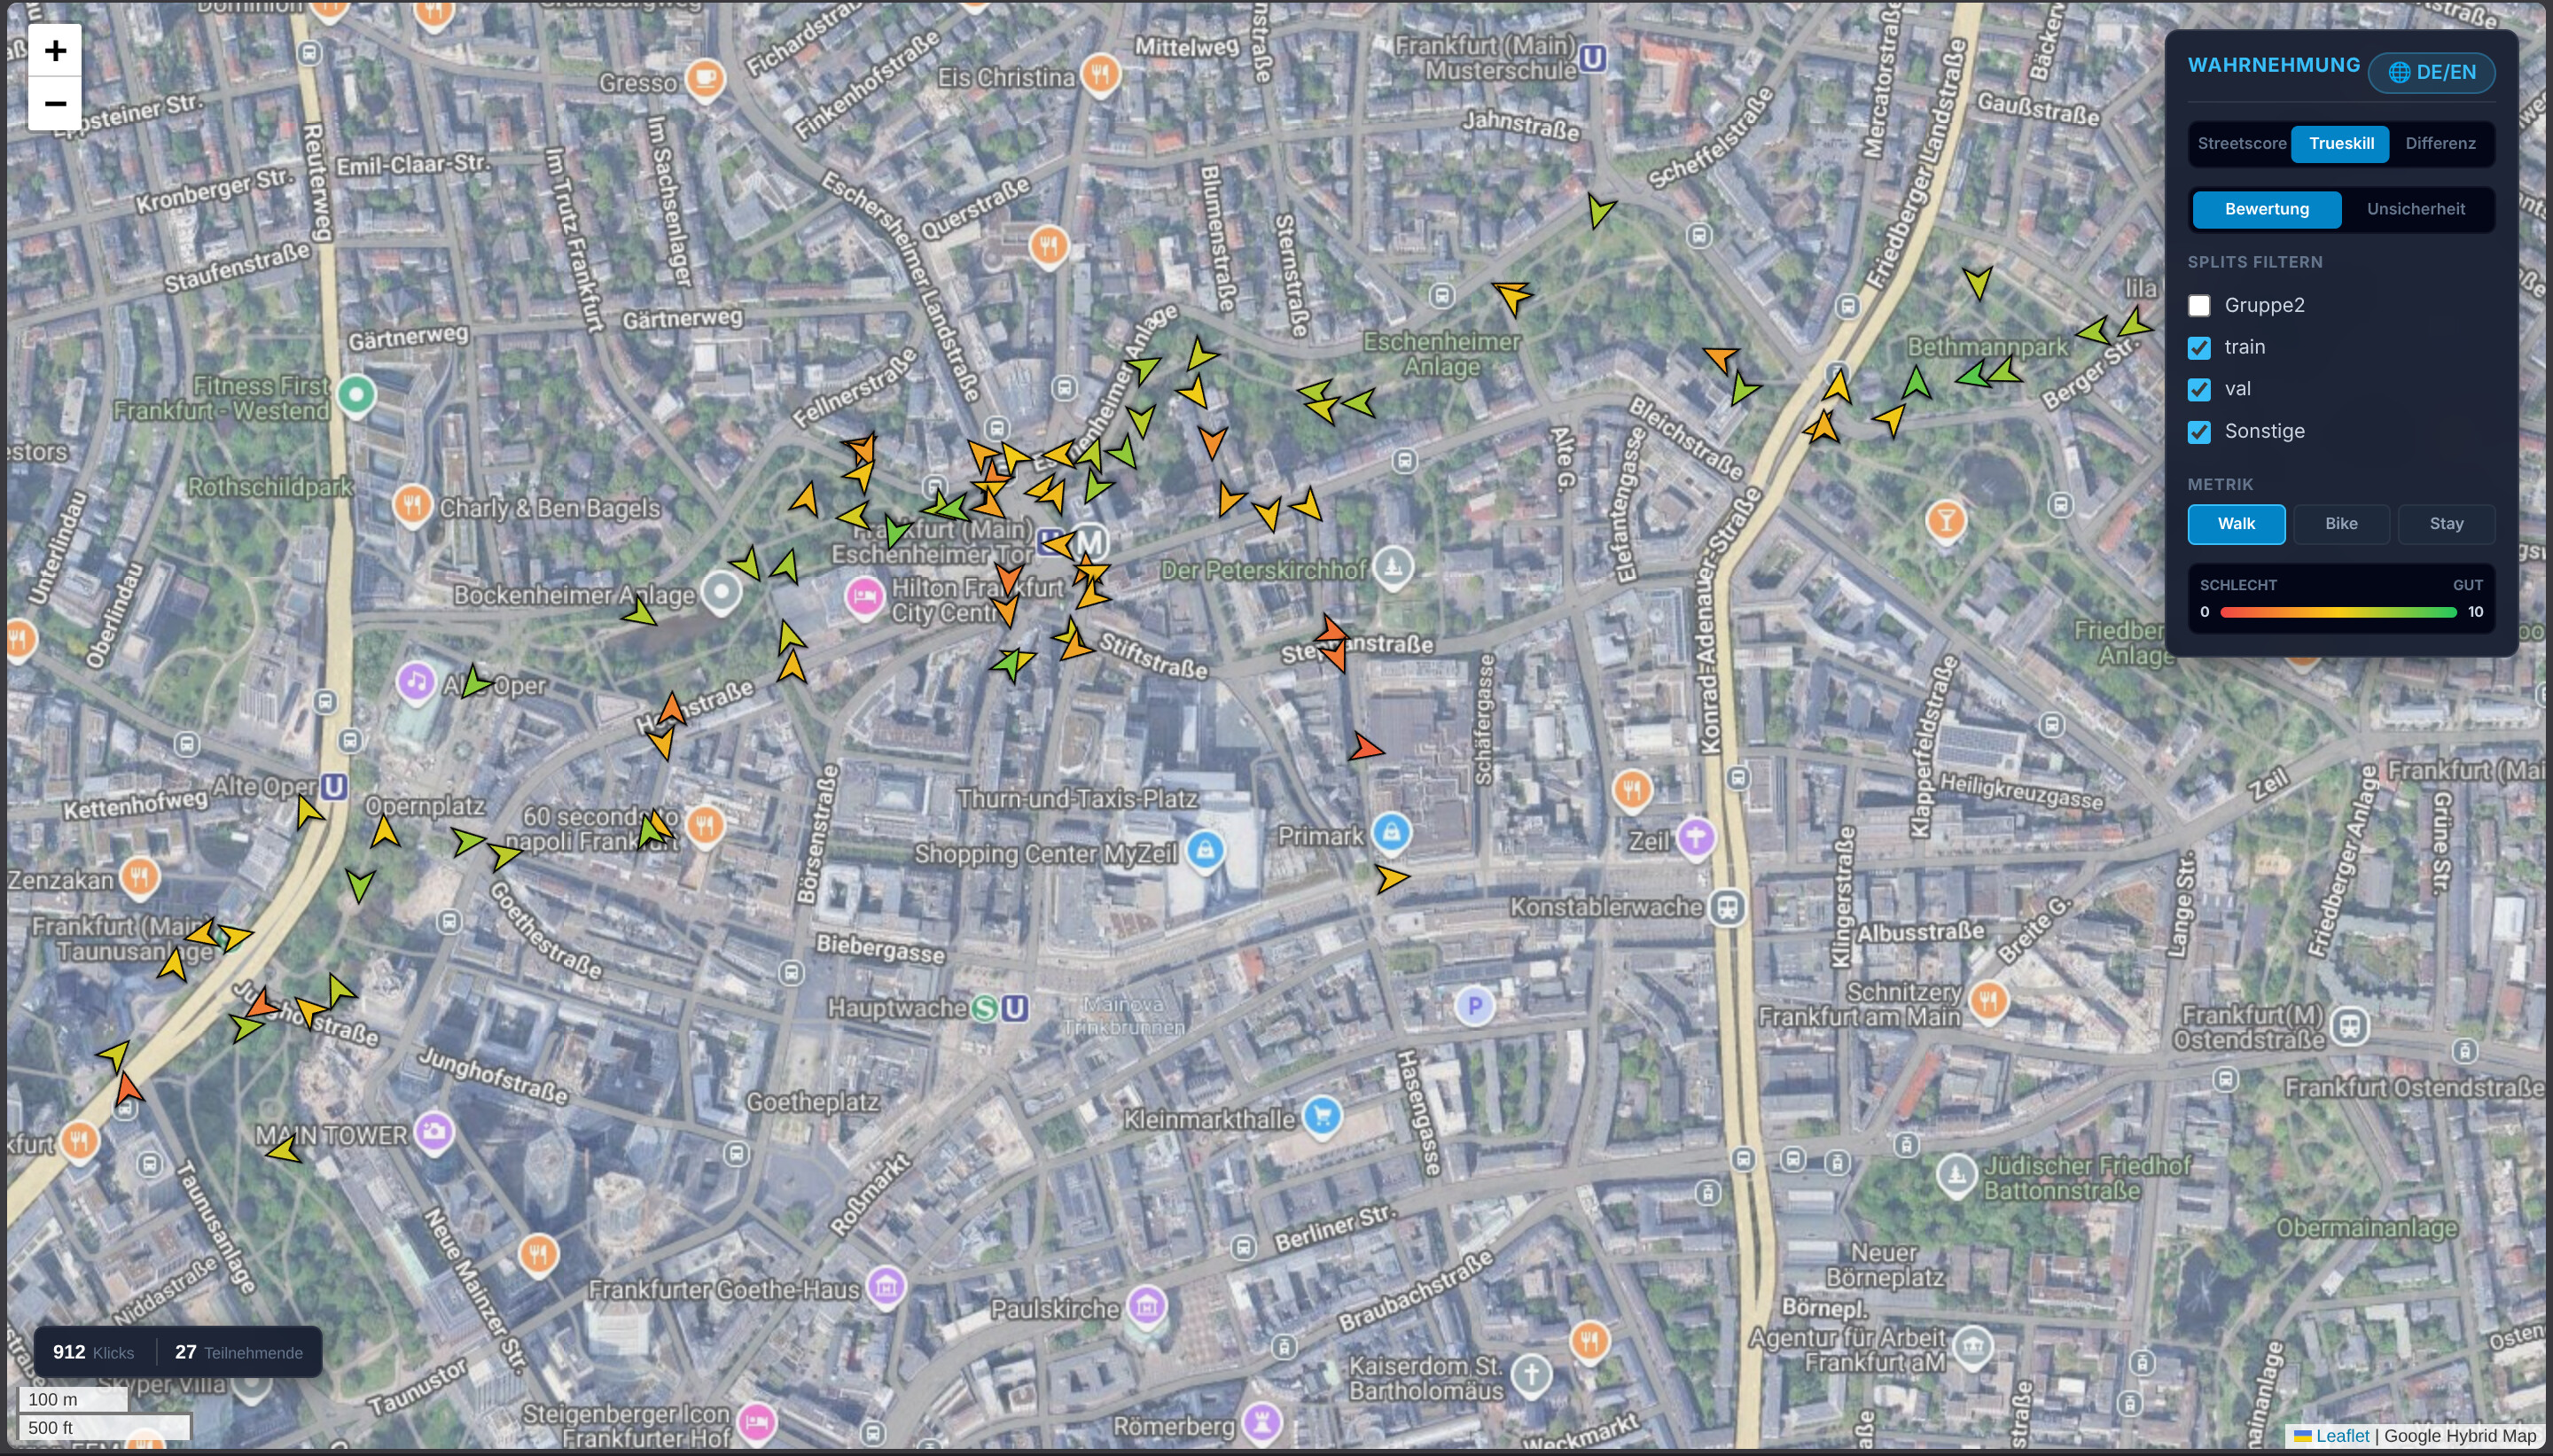
\includegraphics[width=0.85\textwidth]{figures/streetscore_map.jpg}
	\caption[Wahrnehmungskarte des Anlagenrings]{Karte aller im Rahmen der Feldstudie erhobenen Standorte am Anlagenring mit den zugehörigen Fotografien und den daraus resultierenden Umfrage-Wahrnehmungswerten (TrueSkill $\mu$). Die interaktive Version der Karte ist unter \url{https://miguelurenapliego.github.io/ProjektAnlagenring/ABsurveys/index.html?lang=de} verfügbar (Quelle: eigene Darstellung).}
	\label{fig:streetscore-map}
\end{figure}

Abbildung~\ref{fig:streetscore-map} zeigt alle 138 fotografierten Standorte entlang des Anlagenrings, eingefärbt nach dem aus den Paarvergleichen der Feldstudie resultierenden TrueSkill-Wahrnehmungswert. Dieselbe Karte steht zusätzlich in einer interaktiven Fassung zur Verfügung, in der sich für jeden Standort das zugehörige Bild sowie der Umfragewert direkt einsehen lassen: \url{https://miguelurenapliego.github.io/ProjektAnlagenring/ABsurveys/index.html?lang=de}.

Für die in diesem Bericht vorgestellten Auswertungen verwenden wir ausschließlich die aus den echten Nutzerentscheidungen abgeleiteten TrueSkill-Werte, da nur sie unmittelbar auf beobachtetem menschlichem Urteilen beruhen. Das in Abschnitt~\ref{sec:active-sampling} vorangegangene beschriebene StreetScore-Modell wird an dieser Stelle bewusst nicht zur Bewertung weiterer, ungesehener Bilder herangezogen, sondern dient in diesem Projektstadium vorrangig als Machbarkeitsnachweis: Es zeigt, dass sich ein solches Modell grundsätzlich auf unsere lokal erhobenen Daten trainieren lässt, und eröffnet damit die Perspektive, es künftig auf eine deutlich größere Zahl an Straßenraumbildern anzuwenden, für die keine direkten Nutzerurteile vorliegen, ohne dass dafür erneut eine vollständige Befragung durchgeführt werden müsste.

Die folgenden Mosaike stellen für jede der drei Aktivitäten die jeweils am besten und am schlechtesten bewerteten Bilder aus dem Umfrage-Pool gegenüber.

\begin{longtable}{>{\centering\arraybackslash}p{0.46\textwidth} >{\centering\arraybackslash}p{0.46\textwidth}}
	\caption[Gut/schlecht bewertete Bilder je Aktivität]{Gegenüberstellung der am besten und am schlechtesten bewerteten Straßenraumbilder für die Aktivitäten Zufußgehen, Radfahren und Aufenthalten (Quelle: eigene Darstellung).}
	\label{tab:mosaic-all}\\
	\toprule
	\textbf{Gut bewertet} & \textbf{Schlecht bewertet}\\
	\midrule
	\endfirsthead
	\multicolumn{2}{c}{\tablename\ \thetable{} -- Fortsetzung von vorheriger Seite}\\
	\toprule
	\textbf{Gut bewertet} & \textbf{Schlecht bewertet}\\
	\midrule
	\endhead
	\midrule
	\multicolumn{2}{r}{\small Fortsetzung auf nächster Seite}\\
	\endfoot
	\bottomrule
	\endlastfoot
	\multicolumn{2}{c}{\textbf{Zufußgehen}}\\
	\midrule
	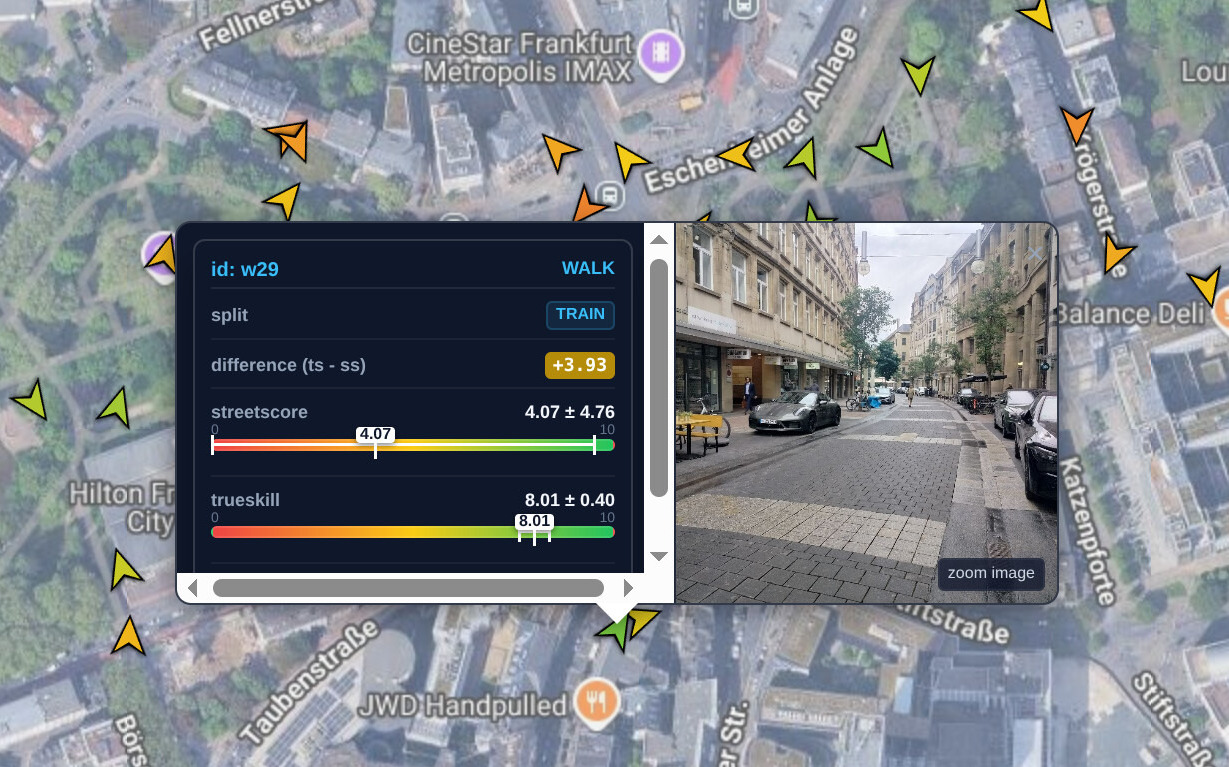
\includegraphics[width=0.9\linewidth]{figures/good_street.jpg} &
	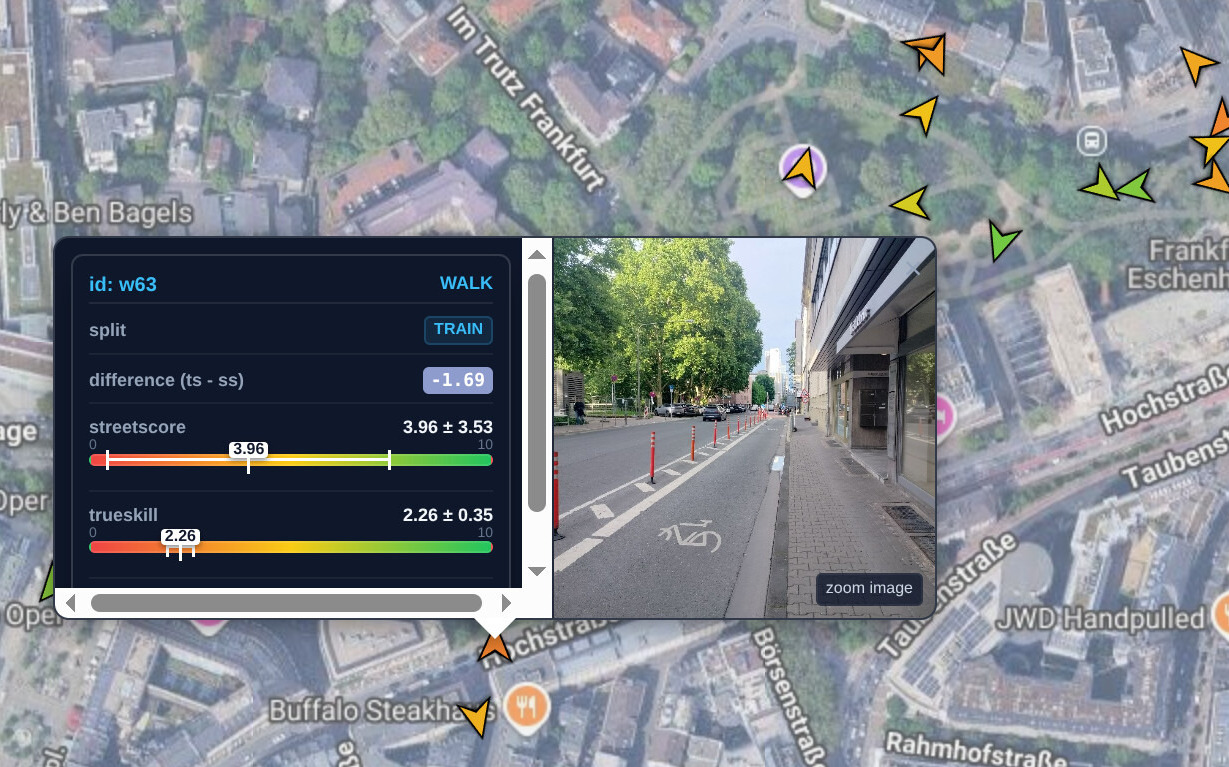
\includegraphics[width=0.9\linewidth]{figures/bad_road.jpg}\\
	\small Zufußgehen -- Bild 1 & \small Zufußgehen -- Bild 1\\[0.8em]
	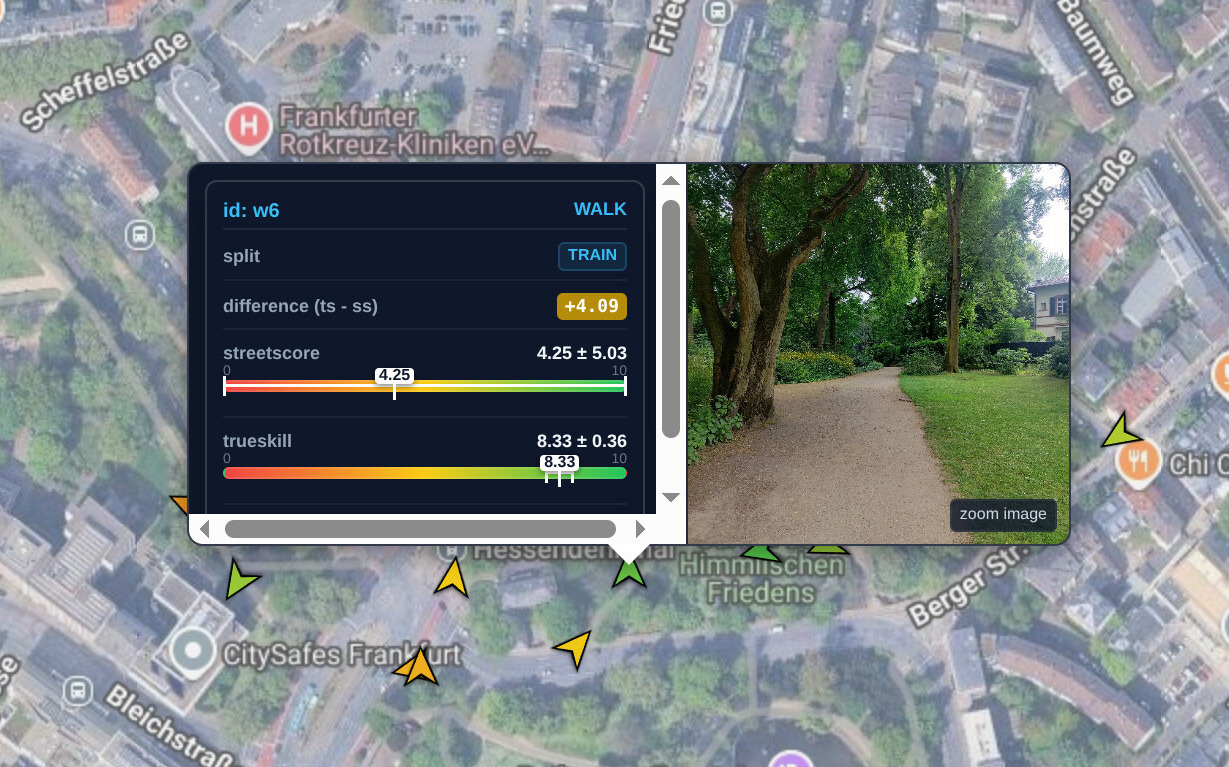
\includegraphics[width=0.9\linewidth]{figures/good_park.jpg} &
	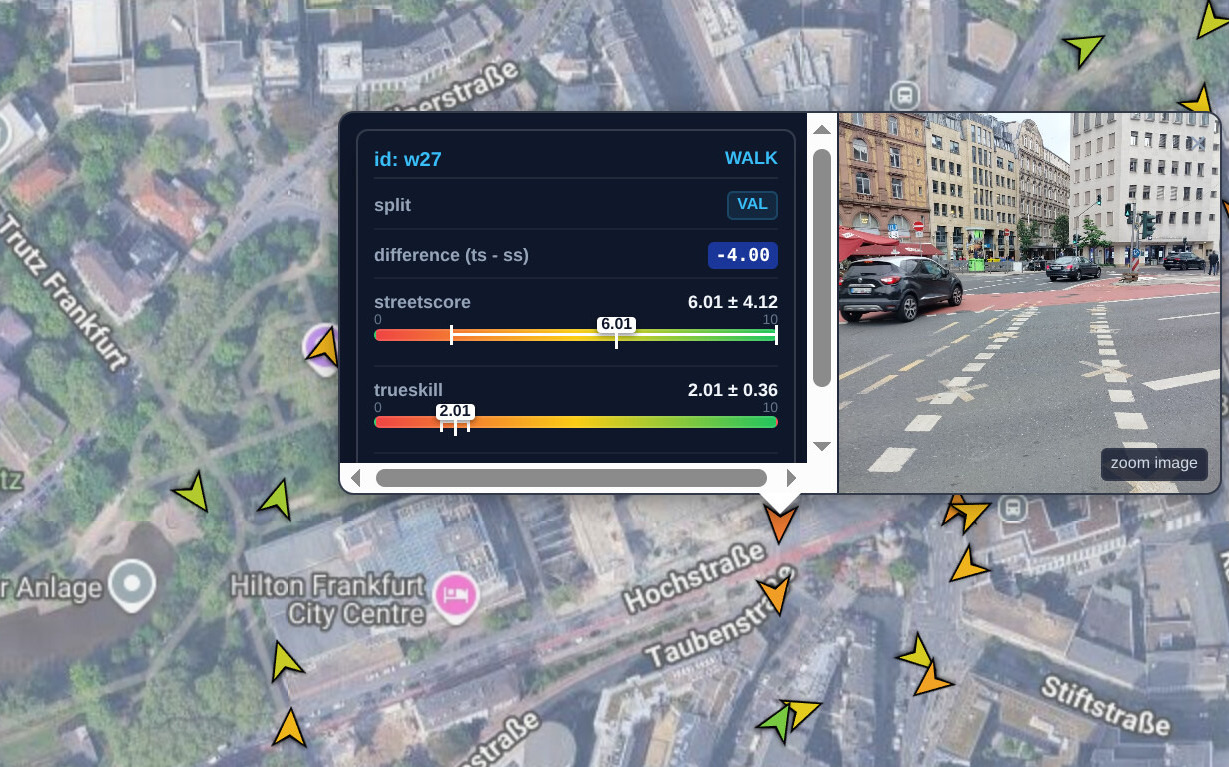
\includegraphics[width=0.9\linewidth]{figures/bad_road_2.jpg}\\
	\small Zufußgehen -- Bild 2 & \small Zufußgehen -- Bild 2\\[0.8em]
	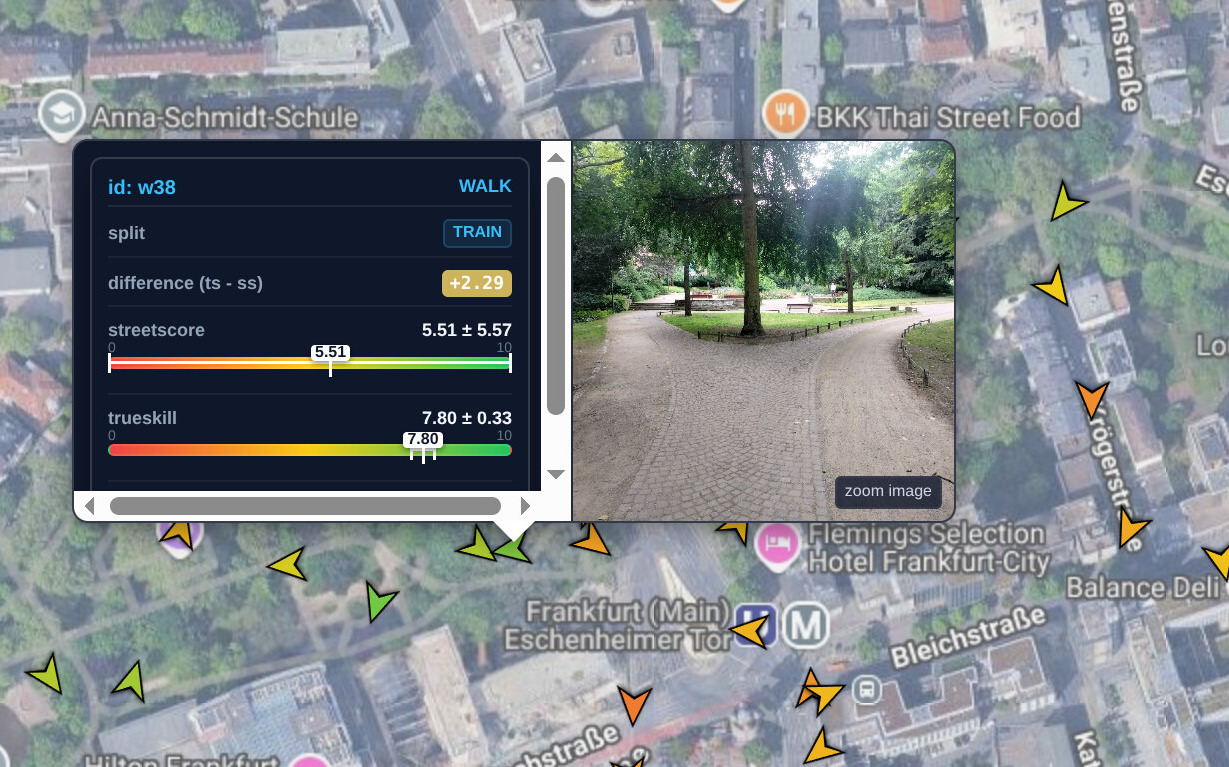
\includegraphics[width=0.9\linewidth]{figures/good_park_2.jpg} &
	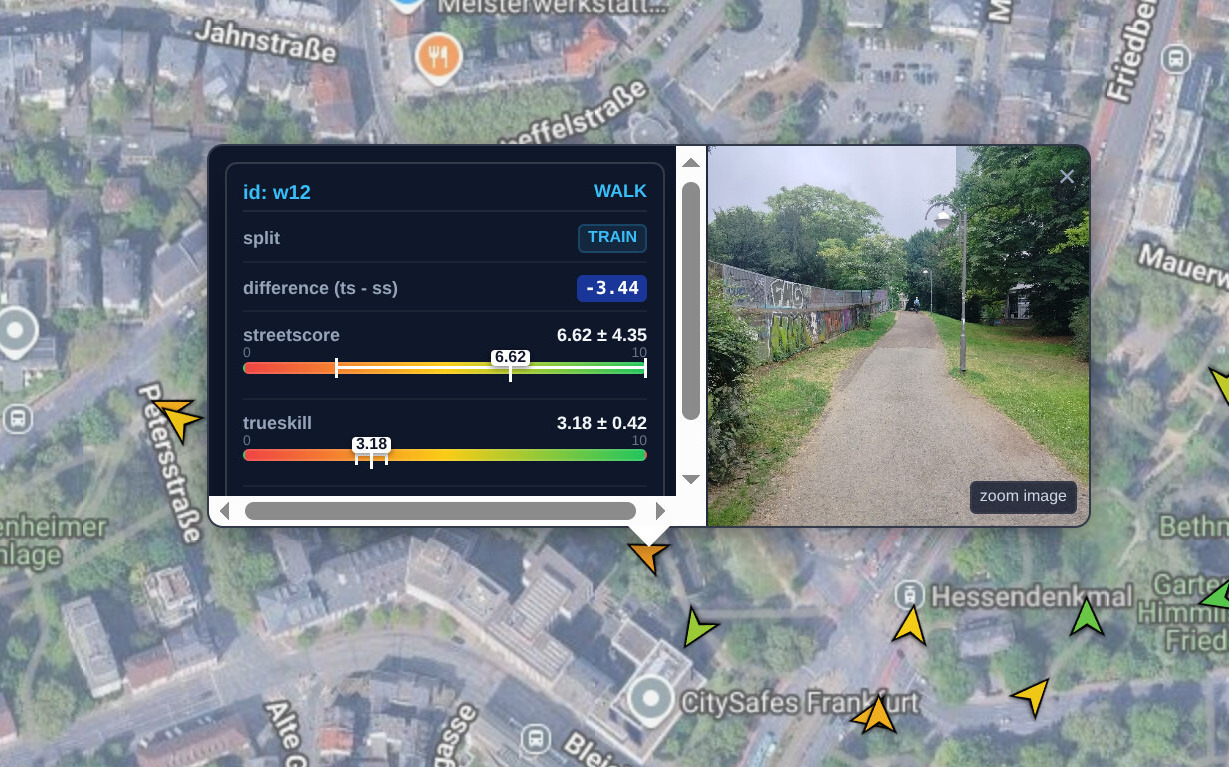
\includegraphics[width=0.9\linewidth]{figures/bad_park.jpg}\\
	\small Zufußgehen -- Bild 3 & \small Zufußgehen -- Bild 3\\[0.8em]
	\midrule
	\multicolumn{2}{c}{\textbf{Radfahren}}\\
	\midrule
	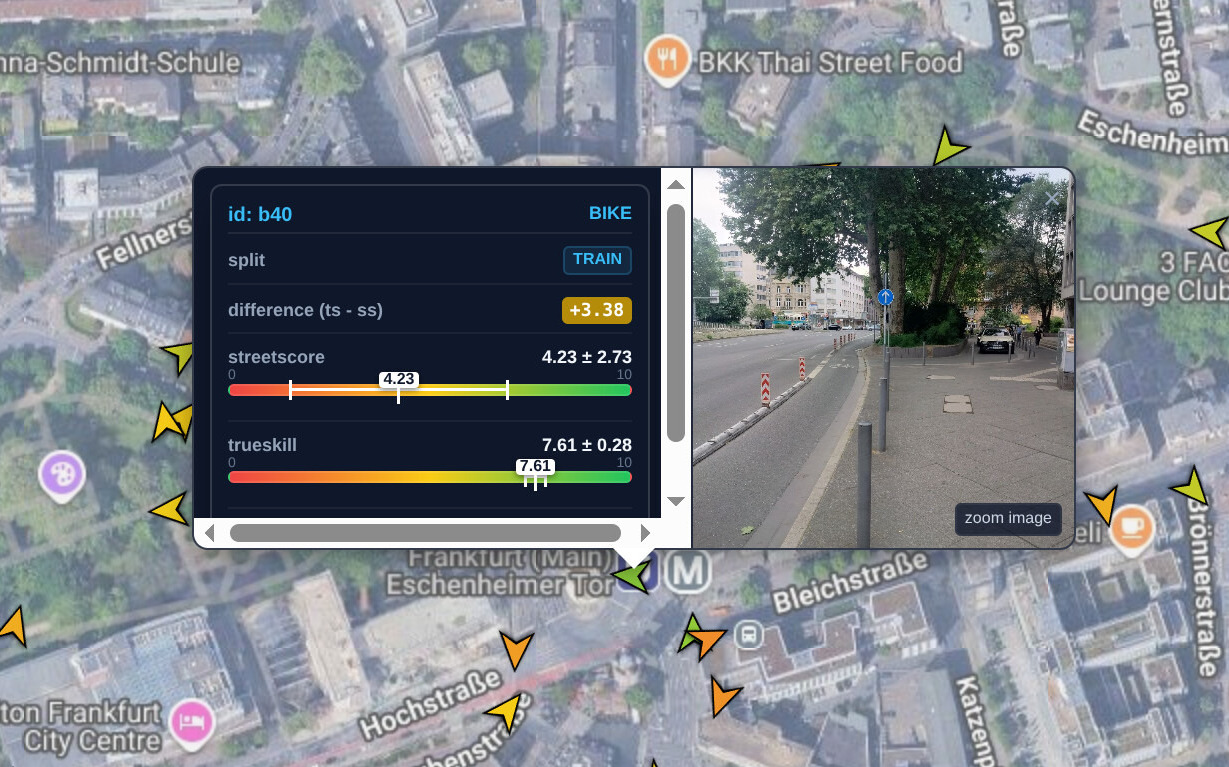
\includegraphics[width=0.9\linewidth]{figures/good_bike.jpg} &
	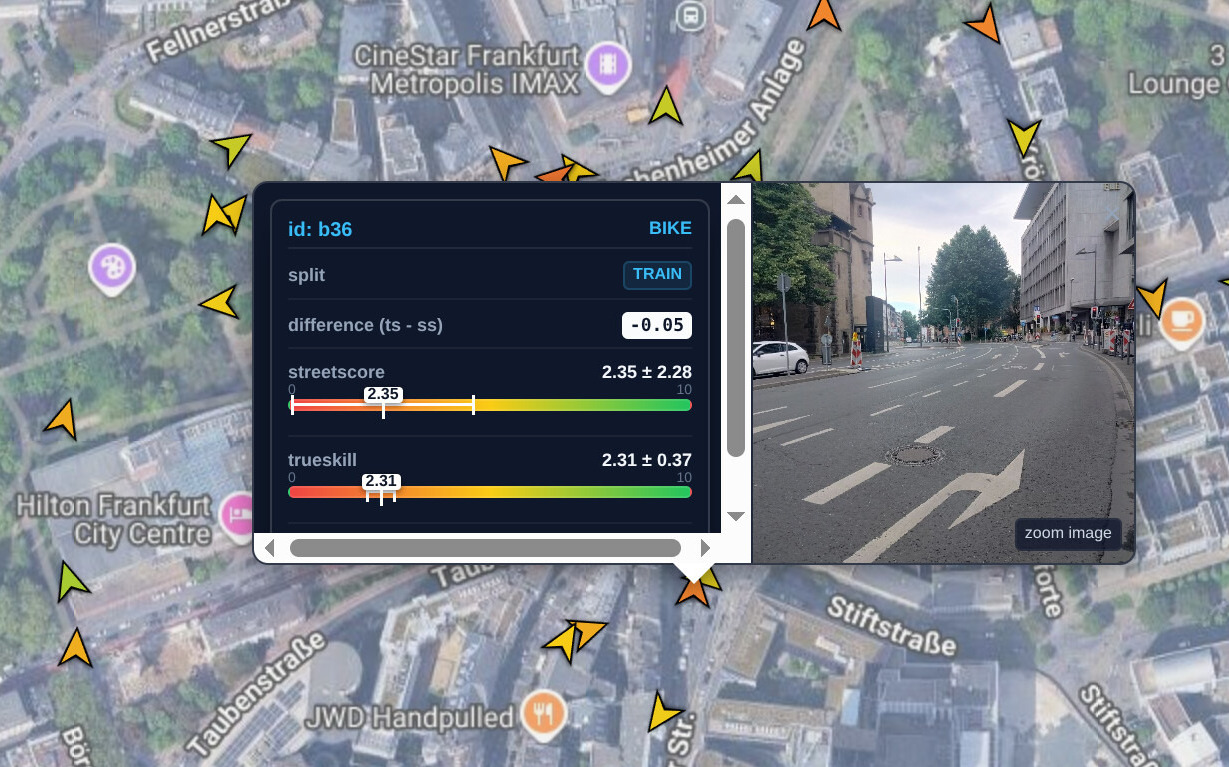
\includegraphics[width=0.9\linewidth]{figures/bad_bike.jpg}\\
	\small Radfahren -- Bild 1 & \small Radfahren -- Bild 1\\[0.8em]
	\midrule
	\multicolumn{2}{c}{\textbf{Aufenthalten}}\\
	\midrule
	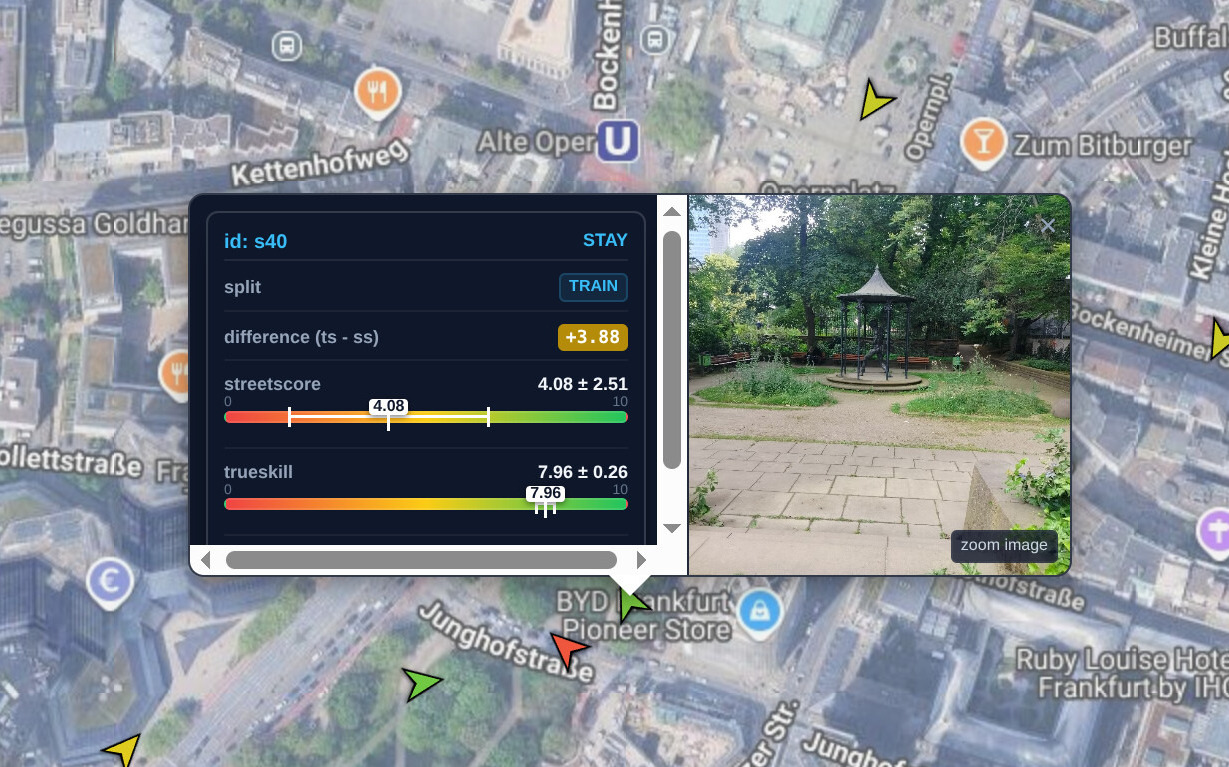
\includegraphics[width=0.9\linewidth]{figures/good_stay.jpg} &
	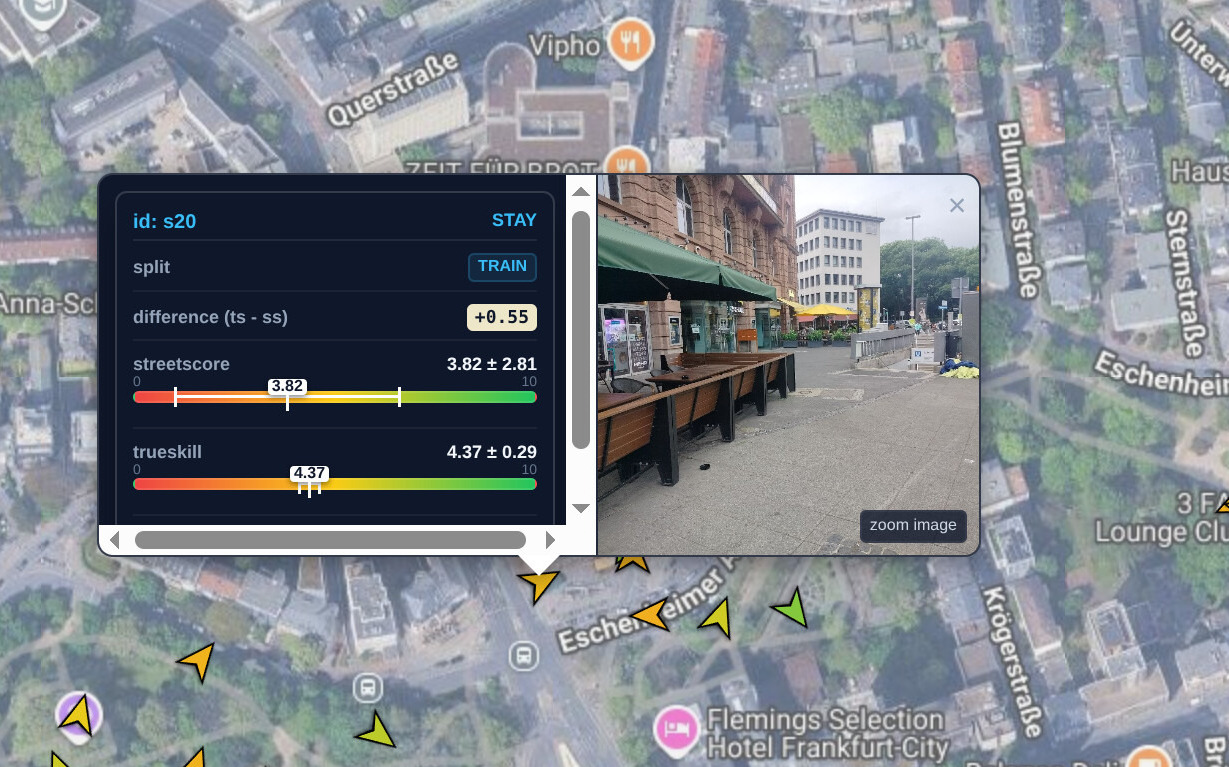
\includegraphics[width=0.9\linewidth]{figures/bad_stay.jpg}\\
	\small Aufenthalten -- Bild 1 & \small Aufenthalten -- Bild 1\\
\end{longtable}

Räumlich zeigt sich in Abbildung~\ref{fig:streetscore-map} ein deutliches Muster: Besonders gut bewertete Orte konzentrieren sich auf den Bethmannpark sowie auf die Cafés und Straßen südlich des Eschenheimer Tors. Demgegenüber wurden einige der großen, verkehrsreichen Kreuzungen am Friedberger Tor, am Eschenheimer Tor sowie rund um die Alte Oper deutlich schlechter bewertet; auch der Fußweg entlang des U5-Tunnels schnitt schlecht ab. Diese räumliche Verteilung legt nahe, dass sehr hochwertig wahrgenommene Teilbereiche des Anlagenrings derzeit von Abschnitten mit schlechter Wahrnehmung umgeben sind. Der Ring wird dadurch nicht als durchgehend zusammenhängender Grün- und Aufenthaltsraum erlebt, sondern in einzelne, voneinander getrennte \enquote{Inseln} guter Aufenthaltsqualität zerlegt, zwischen denen insbesondere die großen Kreuzungen als wahrgenommene Barrieren wirken.

\FloatBarrier
\clearpage
\printbibliography

\end{document}